% \documentclass[10pt, twocolumn]{IEEEtran}
\documentclass[11pt]{IEEEtran}
% \documentclass{llncs}

\usepackage{url}
\usepackage{graphics}
\usepackage{amsmath}

\newcommand{\workingnote}[1]{}        % The version that hides the note.
%\newcommand{\workingnote}[1]{(**#1)}   % The version that makes the note visible.

\renewcommand\url{\begingroup \def\UrlLeft{<}\def\UrlRight{>}\urlstyle{tt}\Url}
\newcommand\emailaddr{\begingroup \def\UrlLeft{<}\def\UrlRight{>}\urlstyle{tt}\Url}

% If an URL ends up with '%'s in it, that's because the line *in the .bib/.tex
% file* is too long, so break it there (it doesn't matter if the next line is
% indented with spaces). -DH

%\newif\ifpdf
%\ifx\pdfoutput\undefined
%   \pdffalse
%\else
%   \pdfoutput=1
%   \pdftrue
%\fi

\begin{document}

%% Use dvipdfm instead. --DH
%\ifpdf
%  \pdfcompresslevel=9
%  \pdfpagewidth=\the\paperwidth
%  \pdfpageheight=\the\paperheight
%\fi

\title{Mixminion: Design of a Type III Anonymous Remailer Protocol}

% Removed for anonymous review
% 
%\author{George Danezis\inst{1} \and Roger Dingledine\inst{2} \and David Hopwood\inst{3}
%        \and Nick Mathewson\inst{2}}
%\institute{Cambridge University
%\email{\emailaddr{george.danezis@cl.cam.ac.uk}}
%\and
%The Free Haven Project
%\email{\emailaddr{{arma,nickm}@freehaven.net}}
%\and
%Independent consultant
%\email{\emailaddr{david.hopwood@zetnet.co.uk}}}
\author{...}
%\institute{}

\maketitle
\pagestyle{plain} 
 
\begin{abstract}
We present Mixminion, a message-based anonymous remailer protocol with
secure single-use reply blocks. Mix nodes cannot distinguish
Mixminion forward messages from reply messages, so forward and reply
messages share
the same anonymity set. We add directory servers that allow users to
learn public keys and performance statistics of participating remailers,
and we describe nymservers that provide long-term
pseudonyms using single-use reply blocks as a primitive. Our design
integrates link encryption between remailers to provide
forward anonymity. Mixminion works in a real-world Internet environment and
requires little synchronization or coordination between nodes.
%, and protects against almost all known attacks.
% ???? Can we say something stronger than 'against almost all known
%      attacks?'  Maybe we can note that we protect against all known
%      attacks at least as well as any other known system with our
%      design parameters. -NM
% we could. suggested phrasing? (how's that? :)
\end{abstract}

\begin{center}
\textbf{Keywords:} anonymity, mix-net, peer-to-peer, remailer, nymserver, reply block
\end{center}

%%%%%%%%%%%%%%%%%%%%%%%%%%%%%%%%%%%%%%%%%%%%%%%%%%%%%%%%%%%%%%%%%%%%%%%

\section{Overview}
\label{sec:intro}

Chaum first introduced anonymous remailers over 20 years ago
\cite{chaum-mix}.
% ???? Did Chaum introduce anonymous remailers?  Weren't there
%      penet-style things before mix-nets? -NM
% no. penet was from the 90's. mix-nets were *way* early. -RD
The research community has since introduced many new
designs and proofs
\cite{abe}\cite{babel}\cite{flash-mix}\cite{kesdogan}\cite{shuffle}\cite{hybrid-mix}, 
and discovered a variety of new attacks 
\cite{back-traffic-analysis}\cite{langos02}\cite{disad-free-routes}\cite{desmedt}\cite{mitkuro}\cite{raymond00}.
But because many of the newer designs require considerable coordination or
synchronization, deployed remailers still use Cottrell's Mixmaster
design from 1994 \cite{mixmaster-attacks}\cite{mixmaster-spec}. Here
we describe
Mixminion, a protocol for asynchronous loosely federated remailers that
maintains Mixmaster's flexibility while addressing the following flaws:

\begin{itemize}
\item \textbf{Replies:} Mixmaster does not support replies or anonymous
recipients --- people who want these functions must use the older and
less secure Cypherpunk Type I remailer design \cite{remailer-history}. We
introduce a new primitive called a \emph{single-use reply block} (SURB),
which makes replies as secure as forward messages. Our design goes a
step further: in Mixminion the remailers themselves cannot distinguish
reply messages from forward messages. We also describe how to securely
build higher-level systems such as nymservers using these SURBs. By
integrating reply capabilities into Mixminion, we can finally retire
the Type I remailer network.

\item \textbf{Forward anonymity:} Mixmaster uses SMTP (normal mail) for
transport. We use TLS over TCP between remailers to encrypt the links,
and use ephemeral keys to ensure forward anonymity for
each message. Link encryption also makes obsolete many active and
passive attacks on the communication links, forcing attackers to run
corrupt nodes for most attacks.

% We also provide flexible delivery schemes ---
%rather than just allowing delivery to mail or Usenet, we allow designers
%to add arbitrary modules to handle incoming and outgoing messages. By
%separating the core mixing architecture from these higher-level modules,
%we can both limit their influence on the anonymity properties of the
%system, and also extend the Mixminion network for uses other than
%anonymous email.

\item \textbf{Exit policies:} Exit abuse is a serious barrier to wide-scale
remailer deployment: most ISPs do not tolerate users who potentially
deliver hate mail, etc. While the original Mixmaster design provided no
way for mixes to advertise their capabilities and roles (so in practice nodes
either allowed all outgoing messages or none), 
%assumed all
%nodes have identical capabilities and roles (and thus messages can exit
%from any node),
Mixminion allows each node to specify and advertise an exit policy. We
describe a protocol which allows recipients to opt out of receiving mail
from remailers, but at the same time makes it difficult for an adversary
to deny service to interested recipients.
% XXXX Actually, Mixmaster allows nodes to -have- different policies:
%      there's just not a good way to advertise your policies beyond 
%      simple capabilities. -NM

\item \textbf{Replay prevention and key rotation:} 
If an adversary records the input and output batches of a mix and then
replays a given message, that message's decryption will be exactly the
same. Thus replayed messages completely break the security of the mix
\cite{chaum-mix}. Mixmaster offers replay prevention by
keeping a list of recent message IDs --- but to keep the list from
getting too long, it expires old entries. The adversary simply has to
wait until the mix has forgotten about a
message before replaying it. Mixminion counters this flaw by introducing
key rotation: a message is addressed to a given key, and after the key
changes no messages to the old key will be accepted; so the mix can forget
about all the messages addressed to old keys. It turns out that the
number of hashes a node needs to remember between key rotations is not
too great a burden.

\item \textbf{Integrated directory servers:} Mixmaster uses several \emph{ad hoc}
approaches to distributing remailer availability, performance, and
key information. But the fact that users and remailers operate with
different information introduces \emph{partitioning} attacks. Mixminion
uses a small group of synchronized redundant directory servers
to provide uniform information about the network.

\item \textbf{Dummy traffic:} Cottrell briefly mentions dummies in
\cite{mixmaster-attacks}, but they are not part of the specification
\cite{mixmaster-spec}. Mixminion uses a simple dummy policy which provably
improves anonymity.

\end{itemize}

%Part of the difficulty in expanding the deployed remailer base is
%due to the liability involved in running a remailer node on the Internet,
%and part is due to the complexity of the current infrastructure ---
%it is fairly hard to add new experimental features to the current software.

We review mixes and mix-nets in Section \ref{sec:background},
describe our goals and assumptions in Section \ref{sec:assumptions},
and then address the above list of improvements in Sections
\ref{sec:design}-\ref{sec:nymservers}. We conclude with a summary of how
our design stands up to known attacks; a list of future
work (remaining tasks we feel confident we can complete);
and finally a list of open questions (unresolved issues for which the
research community currently has no answer).

%The Mixminion Project aims to deploy a cleaner remailer design
%in the same spirit as Mixmaster, with the goals of expanding
%deployment, documenting our design decisions and how well they stand
%up to all known attacks, and providing a research base for
%experimental features.

%Mixminion is a best-of-breed remailer protocol that uses conservative design
%approaches to provide security against most known attacks. The overall
%Mixminion Project is a joint effort between cryptography and anonymity
%researchers and Mixmaster remailer operators. This design document
%represents the first step in peer review of the Type III remailer
%protocol.

% XXXX Mention that we're type-III, and that Mixmaster v4 'will'
%      support type-III? -NM
% i don't think it's a big deal to the academic folk. they certainly
% don't care what some version of some piece of software intends to
% do. let's leave it subtle. -RD

%%%%%%%%%%%%%%%%%%%%%%%%%%%%%%%%%%%%%%%%%%%%%%%%%%%%%%%%%%%%%%%%%%%%%%%

\section{Background}
\label{sec:background}

Chaum introduced the concept of using relay servers, or \emph{mixes},
for anonymous communications \cite{chaum-mix}. Each mix has a public key
which senders use to encrypt messages to it. The mix receives a batch
of these encrypted messages, decrypts them, and delivers them. Because
a decrypted message output looks nothing like the original encrypted
input message,
and because the mix collects a batch of messages and then sends out the
decrypted messages in a new order, an observer cannot learn which incoming
message corresponds to which outgoing message. Chaum showed the
security of a mix against a \emph{passive adversary} who eavesdrops on
all communications but is unable to observe the reordering inside the mix.
Pfitzmann fixed a weakness in Chaum's original scheme based on the
properties of raw RSA encryption \cite{pfitzmann90how}.

However, trusting a single mix is dangerous: the mix itself could be
controlled by the adversary. Therefore users send their messages through
several mixes: if some of the mixes are honest (not run by the adversary),
anonymity will be preserved. In some schemes, such as Mixmaster
\cite{mixmaster-spec} and Babel \cite{babel}, the sender chooses the
mixes that will make up her message's path. Specifically, when Alice
wants to send an anonymous message to Bob through mixes $M_1$, $M_2$,
and $M_3$, she encrypts her message successively with the public keys of
the mixes in reverse order. She includes routing information at each hop,
so that each mix $M_i$ receives the address of $M_{i+1}$ along with the
message intended for $M_{i+1}$ (all encrypted with $M_i$'s public key).
%Recent research on mix networks (mix-nets) includes stop-and-go mix-nets
%\cite{kesdogan}, and schemes based on more sophisticated cryptographic
%constructs that provide robustness \cite{flash-mix}.

A mix network where Alice chooses her route freely from all mixes is
called a \emph{free-route} network. Another approach is a \emph{cascade}
network, where senders choose from a set of fixed paths through the
mix-net. Cascades can provide greater anonymity against an adversary
who owns many mixes \cite{disad-free-routes}, but they are also more
vulnerable to blending attacks \cite{batching-taxonomy} (see Section
\ref{subsec:batching}). Further, cascade networks arguably have lower
maximum anonymity because the number of people Alice can hide among (her
\emph{anonymity set}) is limited to the number of messages the weakest
node in her cascade can handle; a free-route network on the other hand
can create a very high anonymity set because all the traffic does not
need to go through each mix. Mix cascade research includes real-time
mixes \cite{realtime-mix} and web mixes \cite{web-mix}.

More complex designs use zero-knowledge proofs and stronger assumptions
to guarantee delivery or to detect and exclude misbehaving participants.
These include flash mixes \cite{flash-mix} and attacks against them
\cite{mitkuro}, hybrid mixes \cite{jakobsson-optimally}\cite{hybrid-mix},
and provable shuffles \cite{PShuffle}\cite{shuffle}. The properties
of these designs are appealing, but they are often not practical since
they assume a lot of coordination and synchronization between the mixes,
and they impose a heavy computational and communication overhead.

Some mix-net designs allow recipients to construct \emph{reply blocks}
that allow others to send messages to them without knowing their
identities. A reply block contains only the routing portion of a message;
the actual contents are appended by the user who eventually sends a
message to the recipient. In this case the contents are effectively
\emph{encrypted} at each step in the path rather than decrypted.
The recipient knows all the keys used in the reply block and can peel
off all the layers of encryption when the message arrives. Such a design
was first introduced by Chaum \cite{chaum-mix} and later extended in
Babel \cite{babel}. However, Babel's replies are indistinguishable from
forward messages only by passive observers --- the mix nodes can still
distinguish. Babel's reply addresses are also multiple-use, making them
less secure than forward messages due to replay vulnerabilities.

The first widespread public implementations of mixes were produced by the
Cypherpunks mailing list. These ``Type I'' \emph{anonymous remailers}
were inspired both by the problems surrounding the {\tt anon.penet.fi}
service \cite{helsingius}, and by theoretical work on mixes. Hughes
wrote the first Cypherpunk anonymous remailer \cite{remailer-history};
Finney followed closely with a collection of scripts that used Phil
Zimmermann's PGP to encrypt and decrypt remailed messages. Later, Cottrell
implemented the Mixmaster system \cite{mixmaster}\cite{mixmaster-spec},
or ``Type II'' remailers, which added message padding, message pools,
and other mix features lacking in the Cypherpunk remailers.

\subsection{Known attacks against mix-nets}

Attacks against mix-nets aim to reduce the anonymity of users by
linking anonymous senders with the messages they send, by linking
anonymous recipients with the messages they receive, or by linking
anonymous messages with one another \cite{raymond00}.  Attackers may
try to trace messages through the network by observing network
traffic, compromising mixes, compromising keys, delaying messages
so they stand out from other traffic, or altering messages
in transit.  Attackers may attempt to learn a given message's destination
by flooding the network with messages, replaying multiple copies
of a message, or shaping traffic to isolate the target message from
other unknown traffic. Attackers may try to discourage users from
using honest mixes by making them unreliable. They might analyze
intercepted message text to look for commonalities between otherwise
unlinked senders.
Finally, even if all other attacks are foiled, a passive adversary can
mount a long-term \emph{intersection attack} to correlate the times at
which senders and receivers are active \cite{disad-free-routes}.
% Mention that no defense short of N^2 padding is known, and that N^2
% padding doesn't work?

We discuss each of these attacks in more detail below, along with the
aspects of the Mixminion design that provide defense. We provide a summary
of the attacks and our defenses against them in Section \ref{sec:attacks}.

%% try to subvert the process of
%% selecting routes or hiding the correspondence by corrupting mixes, or
%% they try to use side channels containing some information that can be
%% used to link messages together. Finally if none of the above are
%% possible, traffic analysis can take place whereby the flows of messages
%% are processed to find out the most likely recipients or senders. This
%% attack can happen in conjunction with injecting traffic controlled by
%% the attacker.

%% \begin{itemize}

%% \item \textbf{Compromised servers.} The most obvious attack against
%% any system using trusted intermediaries, is for an
%% attacker to corrupt them. This can be done either by the attacker
%% running its own servers, or by hacking into otherwise honest machines
%% or using legal compulsion powers to force them to cooperate and reveal
%% secrets. In order to avoid the possibility that compromised servers
%% would compromise the anonymity of a communication, a series of mixes is
%% used, hoping that at least one of them will be honest.  
%% % XXXX Ick.  With this attack -- and with no other attack -- we
%% %      describe how one ordinarily foils it.   -NM
%% % XXXX Mention explicitly the desired property that if even one 
%% %      server is good, some anonymity is maintained? -NM

%% \item \textbf{Directory-related attacks.} A variant of compromising
%% the core
%% mix servers is to compromise servers making the infrastructure of the
%% network such as the ones responsible for giving out information about
%% the addresses and keys of mixes. An attacker that is able to tamper
%% with this information will be able to divulge wrong information, such
%% as a corrupt subset of the network or wrong keys, that could allow
%% them to compromise the anonymity of the users. % so what do we do
%% 					       % about this?
%% \item \textbf{Partitioning attacks.} In case different messages have
%% some characteristics that can be persistently observed throughout
%% their journey in the network, they can be separated from rest of the
%% traffic and therefore confused with fewer messages. In order to
%% minimize the side channels provided Mixminion hides from all
%% intermediaries information such as their position on the path or the
%% length of the path (although there is a maximium of 32
%% hops). Additionally the forward and reply paths are indistingushable
%% preventing nodes from dividing packets into two distinct
%% categories to partition the anonymity set.
%% %XXXX The fix is early.

%% \item \textbf{Tagging attacks.} An attacker instead of just observing
%% characteristics and side channels in the communications could
%% additionally try to inject some characteristics that he would hope to
%% observe later to trace the message. The simplest way of doing so is by
%% slightly modifying the message, in a way that produces an observable
%% result. Mixminion protects against this attack by making sure that all
%% information that is destined to intermediate mixes has integrity
%% checks, and messages are dropped if they have been modified. All
%% information that is not integrity protected id hidden using random
%% function whose keys should not be known to an adversary. Therefore it
%% should not be possible for him to distinguish between a normal message
%% and a tagged one. Finally the decision was taken that it is better to
%% discard malformed ot tagged messages rather than risk compromising
%% the anonymity of users.
%% % XXXX Fix is early.

%% \item \textbf{Pool attacks.}

%% -delaying
%% -dropping
%% -replay
%% -(n-1) attack

%% -flooding attack
%% -delaying attack
%% -timing attacks
%% \item \textbf{Timing attacks.}
%%\end{itemize}

%%%%%%%%%%%%%%%%%%%%%%%%%%%%%%%%%%%%%%%%%%%%%%%%%%%%%%%%%%%%%%%%%%%%%%%

\section{Design goals and assumptions}
\label{sec:assumptions}

Mixminion brings together the current best practical approaches
for providing anonymity in a batching message-based free-route mix
environment. We don't aim to provide low-latency connection-oriented
services like Freedom \cite{freedom} or Onion Routing \cite{goldschlag99}
--- while those designs are more convenient for common activities like
anonymous web browsing, the low latency necessarily implies smaller
anonymity sets than for slower message-based services. Indeed, we
intentionally restrict the set of options for users: we provide only one
cipher suite, and we avoid extensions that would help an adversary divide
the anonymity set. These assumptions lead to the following design goals.

%While Mixminion protects against known \emph{traffic analysis} attacks
%(where an adversary attempts to learn a given message's sender or receiver
%\cite{rackoff93cryptographic}\cite{raymond00}), we do not fully address
%\emph{traffic confirmation} attacks such as intersection attacks.
%In a traffic confirmation attack, the adversary treats the mix network
%as a black box and observes the behavior of senders and receivers. Over
%time, he can intersect the set of senders and receivers who are active
%at certain times and learn who is sending and receiving which messages
%\cite{langos02}.

% Server requirements
First of all, the system must be relatively simple to deploy. Past systems
have never found it easy to get a reliable group of mix operators to
run long-lived servers. Mixminion must add as few technical barriers as
possible. Thus our protocol uses only loose clock synchronization (within
a few minutes), achieves acceptable performance on commodity hardware,
requires little coordination between servers, and can automatically
handle servers joining and leaving the system.

% Client requriements
Furthermore, software adoption has also been a barrier to past
systems. Thus, only users who receive anonymity from the system must run
special software --- that is, users should be able to receive messages
from anonymous senders and send messages to anonymous recipients with a
standard email client. Users can also send and receive anonymous messages
using only commodity hardware. Finally, although users with persistent
network connections are necessarily more resistant to intersection
attacks than users with intermittent connections, the system must offer
the latter users as much anonymity as possible.

We assume a well-funded adversary who can observe all traffic on the
network, who can generate, modify, delete, or delay traffic on the
network, who can operate mixes of its own, and who can compromise some
fraction of the mixes on the network. Our adversary tries to discover
linkability between sender and receiver, to identify the sender or
receiver of a given message, or to trace a sender forward (or a receiver
backward) to any messages.
%by learning
%(or guessing with a reasonable probability) who is communicating with
%whom. In particular the adversary uses the network traffic patterns to
%trace communication backward or forward and gain additional knowledge
%about communicating partners.

We choose to drop packet-level compatibility with Mixmaster and the
Cypherpunk remailer systems, in order to provide a simple extensible
design. We can retain minimal backwards compatibility by ``remixing''
Type II messages to be Type III messages, thus increasing anonymity sets
in the Type III network. Type II messages travelling between Type III
remailers are treated as plaintext and encrypted to the next remailer
in the chain using its Type III key. The message is sent as a Type III
encrypted message, but it decrypts to reveal the Type II message.

The Mixminion network tries to make it as hard as possible for an
adversary observing the network to gain any additional information
about communicating partners beyond an \emph{a priori} belief. It does
this by providing very little information to outside observers, and
intermediate nodes, to avoid intersection attacks. In particular even
intermediary nodes are not aware of the actual route length (which can
be as long as 32 hops), or their position in the network. Furthermore
the processing for replies is exactly the same as for normal messages
and it is therefore difficult to partition the anonymity sets by
distinguishing between them. 


% replies: we want to avoid partitioning by having reply messages be
%   indistinguishable from forward messages, and just as secure.  To the
%   extent possible, a mix should not be able to learn any more from a
%   message's contents than from the fact of the message's receipt.



%%%%%%%%%%%%%%%%%%%%%%%%%%%%%%%%%%%%%%%%%%%%%%%%%%%%%%%%%%%%%%%%%%%%%%%

\section{The Mix-net Design}
\label{sec:design}

Mixminion uses a free-route mix-net just like \cite{mixmaster-spec}
and \cite{babel}. Mixminion's principal difference from earlier mix-net
designs is the mechanism it uses to support reply messages with the
same processing machinery as forward messages, while at the same time
resisting the attacks described above.

Reusable reply blocks, such as those in the Cypherpunk remailer and
in Babel, are a security risk --- by their very nature they let people
send multiple
messages through them.  These multiple messages can easily be used to
trace the recipient's path: if two incoming batches both include a
message to the same reply block, then the next hop must be in the
intersection of both outgoing batches.  To prevent these replays,
Mixminion therefore provides only \emph{single-use} reply blocks. Since
replies may be very rare relative to forward messages, and thus
much easier to trace, the Mixminion protocol makes reply messages
indistinguishable from forward messages even for the mix nodes. Thus
forward and reply messages can share the same anonymity
set.\footnote{Note that replies are still weaker than forward messages:
an adversary can successively force intermediate mixes to reveal the
next hop of the reply block until its originator is reached.}

The rest of this section describes the mechanism for secure replies,
its integration with the normal sender anonymous message delivery, and
how we defeat tagging-related attacks.  

\subsection{Recipient anonymity and indistinguishable replies}
\label{subsec:replies}
\label{subsec:header-swap}

Mixminion allows Alice to send messages to Bob in one of three ways:

\begin{enumerate}
\item \textbf{Forward} messages where only Alice remains anonymous:
$(A)^x \rightarrow B: M$
\item \textbf{Direct Reply} messages where only Bob remains anonymous:
$A \rightarrow (B)^y: M$
\item \textbf{Anonymized Reply} messages where Alice \emph{and} Bob
   remain anonymous: $(A)^x \rightarrow (B)^y: M$
\end{enumerate}

We denote as $(A)^x$ Alice communicating anonymously under the
pseudonym $x$. In the context of message contents we denote as
$(A)^x_i$ a single use reply block destined to the pseudonym $x$ of
Alice. The subscript $i$ makes explicit the fact that a SURB can only
be used once and a new one has to be used for every communication.

Mixminion's reply
model is in part inspired by Babel \cite{babel}, as it requires the
receiver of a reply block to keep no other state than its secret keys,
in order to read the reply.  All the secrets used
to strip the layers of encryption are derived from a master
secret contained in the last header of the single-use reply block, which
the creator of the block addresses to itself and encrypts under its
own public key.

By making forward messages and replies indistinguishable even to mixes,
we prevent an
adversary from dividing the message anonymity sets into two classes. In
particular, if replies are infrequent relative to forward messages,
an adversary who controls some of the mixes can more easily trace the
path of each reply.

Having indistinguishable replies, however, makes it more difficult to
prevent tagging attacks.  Since the author of a reply block is not the
one writing the payload, a hash of the entire message cannot be used.
Therefore, since we choose to make forward messages and replies
indistinguishable, we cannot include hashes for forward messages either.
Our approach to defending against these attacks is discussed in more
detail in Section \ref{subsec:tagging-defenses}.

We require parties that benefit from anonymity properties to run dedicated
software.  Specifically, senders generating forward messages must be able
to create onions, and anonymous receivers must be able to create reply blocks
and unwrap messages received through those reply blocks. Other parties,
such as those receiving forward messages and those sending direct reply
messages, do not need to run new software. We use the quoting
performed by ordinary mail software to include the reply
block in a direct reply; this is sent to a node at the Reply-To:
address, which extracts the reply block and constructs a properly
formatted onion.

\begin{figure}
\begin{center}
\resizebox{15cm}{!}{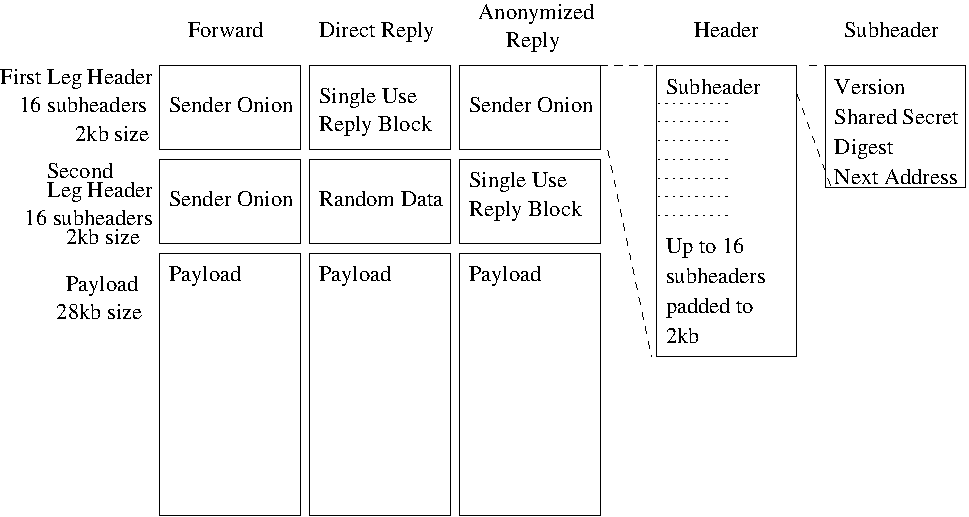
\includegraphics{headerDiagram}}
\caption{The header configurations for different anonymity functions.} 
\end{center}
\end{figure}

Messages are composed of a header section and a payload. We divide
a message's path into two \emph{legs}, and split the header section
correspondingly into a main header and a secondary header. Each header
is composed of up to 16 subheaders, one for each hop along the path.
Each subheader contains a hash of the remainder of its header as
seen by that mix, so we can do
integrity-checking of the path (but not the payload) within each leg.
Each subheader also contains a symmetric key, which is used to derive a
decryption key for decrypting the rest of the message. The mix also
derives a padding seed from this master key. It uses this padding seed
to place predictable padding at the end of the header, so the hash will
match even though each hop must regrow the header to maintain constant
length. Each subheader also includes the address of the next node to which
the message should be forwarded, along with its expected signature key
fingerprint --- the mix refuses to deliver the message until the next
hop has proved its identity.

For forward messages, Alice provides both legs. For anonymous replies, Alice
uses Bob's reply block as the second leg, and generates her own path
for the first leg.  To send a direct reply, Alice can use an empty
second leg, or send the reply block and message to a mix that can wrap
them for her. Figure 1 illustrates the three options.

When Alice creates her message, she encrypts the secondary header
with a hash of her payload (as well as the usual layered onion
encryptions). Alice's message traverses the mix-net as normal (every
hop pulls off a layer, verifies the hash of the current header,
and puts some junk at the end of the header), until it gets to a
hop that is marked as a \emph{crossover point}. This crossover point
performs a ``swap'' operation: it decrypts the secondary header with
the hash of the current payload, and then swaps the two headers. The
swap operation is detailed in Figure 2 --- specifically, the normal
operations done at every hop are those above the dotted line, and the
operations performed only by the crossover point are those below
the dotted line. The encryption primitive, labeled ``LBC'', that is
used to blind the second header and the payload needs to have certain
properties:

\begin{itemize}
\item it is length-preserving;
%\item it behaves like an all-or-nothing transform on the whole of
%      the message;\footnote{Except that we need a keyed primitive,
%      whereas an all-or-nothing transform is normally unkeyed, and
%      not length-preserving.}
%% I think that if we have the next item, we don't need this. -DH

\item it should be impossible to recognize the decryption of a modified
      block, without knowledge of the key;
%what the heck does this mean? i don't know what 'the key' is. this is
%probably too imprecise for us.
\item it should be equally secure to use the decryption operation
      for encryption.
\end{itemize}

To fulfill the above requirements we use a variable length block
cipher adapted to the length of the payload; that
is, a cipher that acts as a permutation on a block the size of its
input (a header or the payload).  Possible candidates
include LIONESS \cite{BEAR-LIONESS} and SPC \cite{SPC}.
The cryptographic property required is that of a super-pseudo-random
permutation (a.k.a. strong pseudo-random permutation) or SPRP \cite{sprp}.\footnote{
The weaker PRP property may be sufficient, given that preventing
replays limits the number of oracle queries to 1; this will need
further analysis.  In that case the simpler BEAR construction
\cite{BEAR-LIONESS} could be used instead of LIONESS.}
Thus if any bit of
the encrypted material is changed, the decryption will look like random
bits.  An SPRP is also equally secure in the encryption and decryption
directions.  Below we describe
how this approach helps protect against tagging.

% BEAR isn't an SPRP; LIONESS is. I'm not sure that an SPRP is necessary,
% but I'm sure that it is sufficient. We don't need encryption and
% decryption to be the same. -DH

%To fulfill the above requirements we use a variable block size block cipher
%named BEAR [2] as our encryption and decryption primitive. BEAR offers the
%property that if any bit of the encrypted material is changed, the decryption
%will look like random bits. We can use BEAR in a mode where decryption and
%encryption are equivalent, by using the same key for both of its hash steps.
%
% ``Both hash steps''?  We never mention Bear's hash steps... -Nick
% True. Does adding 'its' help? -RRD
% Adding 'of' helps more for me.  Also, doesn't George once have a
% source for this? -Nick


\begin{figure}
\begin{center}
\resizebox{10cm}{!}{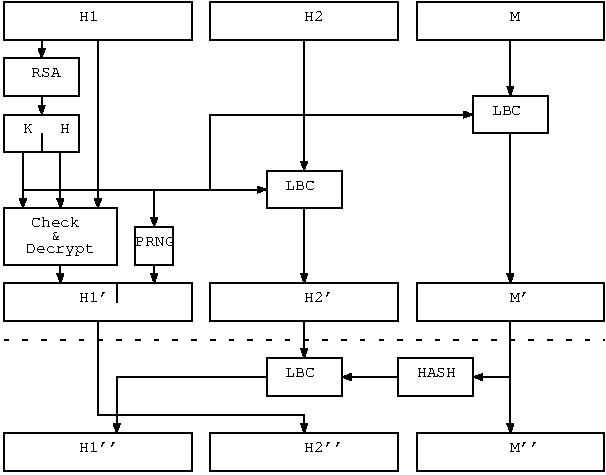
\includegraphics{SWAP}}
\caption{The operations required by the ``swap'' method} 
\end{center}
\end{figure}

\subsection{Defenses against tagging attacks}
\label{subsec:tagging-attacks}
\label{subsec:tagging-defenses}

To motivate the Mixminion design, we describe an attack
that works against many mix-net protocols, including Mixmaster and Babel.

A {\em tagging attack} is an active attack in which a message is
modified by altering part of it (for example by flipping bits), so
that it can be recognized later in the path.  A later mix controlled by
the attacker can recognize tagged messages because the header or the
body does
not conform to the expected format when decrypted.  Also, the final
recipient can recognize a tagged message for which the payload has
been altered.

Checking the integrity of hop headers individually is not
sufficient to prevent tagging attacks.  For example, in Mixmaster
each hop header contains a hash of the other fields in that header
\cite{mixmaster-spec}.
Each mix in the path checks the integrity of the header, and drops
the message immediately if it has been altered.  However, 
an attacking mix can still alter a header that will be decrypted
only after several more hops, and so tagging attacks are still possible.

The most straightforward way to prevent tagging attacks is to
verify the integrity of the whole message at every hop.  For forward messages,
then, the padding added to a message must be derived deterministically,
so that it is possible to calculate
authentication tags for the whole message at each hop.  But
the situation becomes more complicated when reply messages are
introduced --- the message and the reply block are
created by different users. It is impossible for the creator
of the SURB to include in the header a checksum of a message he
does not yet know. Therefore techniques taken straight out of modern
cryptology, such as semantically secure or randomized encryption, that
make sure an adversary does not gain any information by sending
malformed messages to the mix (since the mix acts as a decryption oracle),
cannot be used.

Mixminion uses a hybrid strategy to protect against
such attacks: we use cryptographic checksums to protect the headers,
and we make sure that the addressing information contained in the
headers is destroyed if the payload is modified by an adversary.

If the Mixminion design did not require
the crossover point, an adversary could mount a tagging
attack by modifying the payload of a forward message as
it leaves Alice, and recognizing it later when it reaches Bob.
Specifically, if our encryption mechanism were an ordinary
counter-mode cipher, he might alter a specific byte in the payload of
a message entering the mix-net. Since many of the outgoing messages
will be in part predictable (either entirely plaintext, or with
predictable PGP header material), the adversary can later observe
messages exiting the mix-net and look for payloads that have a
corresponding anomaly at that byte. Other block cipher modes such as
Cipher Block Chaining (CBC) present comparable problems, since whole
blocks would look like random noise instead of the normal payload.

We use a large-block cipher as described in the previous section to
minimize the amount of information an adversary can learn from tagging.
If he tags a message
leaving Alice, the payload will be entirely random when it reaches
Bob.  Thus, an adversary who tags a message can at worst turn the
corresponding payload into trash.  
%%Thus if he tags more than one message in the entire mix-net, he
%%learns only one bit from each tagged message, so he cannot distinguish
%%the tagged messages. 
% I think that the above sentence raises more objections than it 
% addresses; thus, I'm omitting it.  The real security comes from the
% crossover step as described below.  Without the crossover
% decryption, BEAR is insufficient, and one bit is too much. -Nick
%Nevertheless, this may still allow an adversary to
%break anonymity in some cases.

We briefly considered introducing \emph{cover-trash}, dummy messages
designed to look like tagged messages, to frustrate
these tagging attacks; but that problem is as complex as the dummy
traffic problem \cite{langos02}. Instead, we use the
``swap'' step at the
crossover point to prevent the attacker from learning information from
tagging attacks. The second header of the message, that contains the
path to the final destination of the forward path, is encrypted by the
sender with the hash of the payload that is to arrive at the mix. The
mix then needs to perform the decryption and swap the first header for
the second one.
Our security argument has three cases:

\begin{itemize}
\item Forward messages: if the message is tagged during the first leg,
the second header is unrecoverable, and so the adversary cannot
learn the intended destination of the message. If the message is tagged
during the second leg, then the first leg has already provided anonymity,
and so the adversary cannot learn the sender.
\item Direct reply messages: since the decryption algorithm provides
secrecy equivalent to encryption, the effect is similar to {\em encrypting}
the payload at each step along a reply block. Only the recipient can learn,
after peeling off all layers, whether the message has been tagged. Thus
tagging attacks are useless against direct reply messages.
\item Anonymized reply messages: as with forward messages, if the first leg
is tagged the second header is unrecoverable --- so an adversary will
never learn that the message was addressed to a reply block. And as with
direct reply messages, only the recipient can learn if the second leg is
tagged.
\end{itemize}

While direct reply messages do not need a crossover point in the path
(the adversary can never observe his tag), forward messages still need a
crossover point to prevent end-to-end tagging. But since the first leg
either provides sufficient anonymity or destroys the information about
the second leg, the second leg in a forward message can be very short.
At the extreme, the first hop in the second header could directly
specify the message recipient. However, the choice of crossover point
can still reveal information about the intended recipient,\footnote{For instance,
some mixes may only allow outgoing mail to local addresses; if such a
node gets a crossover message that has been trashed, it might guess
that the recipient is one of the local addresses.} and so we recommend
that the second leg be at least a few hops long.
We use a path length of 4 hops per leg, but with only 2 hops in the
second leg of a forward message.

It is worth noting that while semantically secure encryption cannot be
used directly to solve the problem of tagging attacks in Mixminion, the
structure of the operations performed on the message as it travels
through the network is very similar to the Luby-Rackoff \cite{sprp}
structure. In particular the fact that the header depends on the body
and \emph{vice versa} makes sure that if the message is tagged in
any way it will become entirely different from what was intended, and
its contents
will provide no information at all to an attacker. It is the
first time, to our knowledge, that this property is achieved by
distributing the operation of a cipher across many nodes of a mix network.

No mix except the crossover point can get any information distinguishing
forward messages from replies. While the crossover point cannot be
certain whether the message that it is processing is a forward message
or a reply, it does gain partial information because crossover points
are less frequent on forward paths, and therefore a message which is
crossing-over is more likely to be a reply message.

\subsection{Multiple-message tagging attacks}
\label{subsec:multi-tagging}

The above design is still vulnerable to a subtle and dangerous
attack. If Alice sends a group of messages along the same path, the
adversary can tag some of those message as they leave Alice, recognize
the pattern (number and timing of tagged and untagged messages) at the
crossover point, and observe where the untagged ones go.
% (if he built
%the second leg himself, as in an anonymized reply, he can recognize
%it immediately).
With some assumptions about our adversary, we can reduce
this attack to a traffic confirmation attack we're already willing to
accept: when Alice sends a bunch of messages, the adversary can count
them and look for the pattern later. He can also drop some of them and
look for resulting patterns.

The adversary can only recognize a tag if he happens to own the crossover
point that Alice chooses.
Therefore, Alice picks $k$ crossover points for her
messages;\footnote{
  We can prevent the adversary from using divide-and-conquer on Alice's
  groupings if Alice uses a hybrid path starting with a short cascade ---
  so even if the adversary tags a subset of the messages he doesn't know
  (unless he owns the whole cascade) the groupings of tagged messages.
}
to match a tag signature with certainty an adversary would
have to own all $k$ crossover points.  (And even then, it seems harder
as the subsets of her messages would overlap with subsets of
messages from other senders.)

% The argument above seems a little handwavy to me.  We should either
% expand it to say why the adversary needs certainty to mount the
% multiple-messages attack, or express less confidence in it.  I'm
% taking the latter route below, and changing ``is infeasible''
% to ``seems infeasible''  -Nick

The key here is that when the adversary doesn't own a given crossover
point, tagging messages destined for that crossover is equivalent to
dropping them.  The crossover point in question simply doesn't deliver
the message to the second leg. Therefore, if the adversary doesn't own
most of the crossover points that Alice chooses, a successful
multiple-message tagging attack seems infeasible.  We leave a security
analysis of the multiple-paths idea to future work; but see
Section \ref{sec:maintaining-anonymity}.

\section{Related design decisions}

%In this section we discuss how we are using
%link encryption with ephemeral keys to provide forward anonymity,
%message types and modules to handle different types of messages, and
%exit policies for advertising what delivery options a node will provide.

\subsection{Link encryption and what it gets us}
\label{subsec:link-encrypt}

Unlike remailer Types I and II that used SMTP \cite{SMTP} (i.e. ordinary
Internet e-mail) as their underlying transport mechanism, Mixminion
clients and nodes communicate using a forward secure encrypted channel
based on TLS \cite{TLS}.  
TLS allows the establishment of an encrypted tunnel using ephemeral
Diffie-Hellman keys. In order to guarantee that the receiving end is
the one intended by the creator of the anonymous message, the
receiving node signs the ephemeral key. As soon as a session key
has been established, the parties destroy their Diffie-Hellman keys
and begin sending messages through the tunnel. After each message, the
parties perform a standard key update operation to generate a fresh
key, and delete the old key material.  Key updates don't require any
asymmetric encryption techniques, so they are relatively fast.

% Do we want to specify how much of the above happens with TLS
% Handshake/ChangeCipherSpec packets, and how much happens within the 
% application data?  I =believe=[*] that TLS can do all of the above with 
% standard stuff; do we want to use TLS vocabulary to convince
% people? 
%
%  [*]My only reservation is doing key updates without assymetric
%  encryption.  I need to doublecheck that such an operation is really 
%  specified in the RFC.                               -Nick
%  It is: the server can send a HelloRequest or the client a
%  ClientHello at any time. -DH.


% Also, do we want to specify a required level of encryption?  It
% would be pretty useless if we allowed export or null ciphers
% suites.
%
% One of these modes (specified in ietf-tls-ciphersuite-03.txt) is
% probably best for us:
%             (A)   ``DHE-DSS-AES128-SHA''
%             (A)   ``DHE-RSA-AES128-SHA''
%             (B)   ``ADH-AES-128-SHA''
%             (A)   ``DHE-DSS-AES256-SHA''
%             (A)   ``DHE-RSA-AES256-SHA''
%             (B)   ``ADH-AES256-SHA''
% I'm not sure, though, whether we want one of the cert-based ones (A)
% or one of the the anon-server ones. (B) -Nick

The purpose of link encryption is to provide forward secrecy: 
after the keys have been deleted, not even the
nodes that exchange messages can decrypt or recognize messages
that might have been intercepted on the links. This makes it
impossible to comply with decryption notices of past traffic 
that might be served in
some jurisdictions.  
%It also forces adversaries to 
%corrupt and control nodes in order trace
%a forward anonymous communication by requesting nodes to decrypt
%it. 
%   I removed these sentences. If somebody knows what we meant,
%   feel free to fix that. :) -RRD
% In advance, or later?  I'm not clear what the above sentence is
% saying. -Nick
%(Reply blocks can still be used for this purpose.)
Even if an
attacker manages to get hold of the session key at a particular point
he would have to observe all subsequent traffic to be able to update
his key appropriately.

Additionally link encryption makes active and passive attacks on the
network links more difficult. Given that mix messages give an
indication to the mixes about the identity of their successors it is
hard for an 
adversary to modify messages, inject messages to a node as if they
were part of the normal communications, or delete messages.
An additional \emph{heartbeat} signal in the SSL tunnel complicates
message delaying attacks.
%This forces a
%determined adversary to run nodes or to corrupt nodes in 
%order to break the anonymity of Mixminion.
%  hogwash. the adversary can muck up the network link, and we can't
%  distinguish that from normal network suckage -RD

The encrypted channel offers only limited protection against traffic
analysis. Encrypted links between honest nodes prevent an adversary
from recognizing even his own messages; but without link padding, he
can still measure how much traffic is being transmitted.

As a fringe benefit, using a separate link protocol makes it
easier to deploy relay-only mixes --- such nodes simply omit SMTP
support.  (See Section \ref{subsec:delivery-modules} below.)
% Credit for the above point goes to Len.

\subsection{Message types and delivery modules}
\label{subsec:delivery-modules}

%XXXX
[I think it is important to say what modules get us in comparison to
normal client side Mixminion (which servers can also use). In
particular, access to some shared key material and plug-in for
infrastructure critical services. -GD]

Once a Mixminion packet reaches the final mix in its path, it must
either be delivered to its intended recipient, dropped if it is an
intra-network dummy message, or processed further if it is a remixed
Type II packet. In order to support different kinds of
delivery, the header includes a type code for the action to be taken
to deliver the message.  A few types --- such as `dummy', `SMTP', and
`local delivery' --- are specified as a part of the Mixminion
standard.  Others may be added by future extensions, to
implement abuse-resistant exit policies (see Section
\ref{subsec:exitpolicies}), to administer nymservers (see Section
\ref{sec:nymservers}), to publish anonymously to Usenet, to relay
messages to older remailers, or to support other protocols.

Nearly all delivery methods require additional information beyond the
message type and its payload.  The SMTP module, for example, requires
a mailbox.\footnote{A {\it mailbox} is the canonical form of the
``{\tt user@domain}'' part of an e-mail address. Mixminion uses only
mailboxes in the protocol, because the display name and comment parts
of an e-mail address could potentially be different for senders who
have obtained an address from different sources, leading to smaller
anonymity sets.}
This information is placed
in a variable-length annex to the final subheader.

%\footnote{It must be
%in the header, since putting delivery information in the payload would
%prevent people from creating SURBs that can be delivered by SMTP.
%On the one hand, under the ``header swap'' method described in
%\ref{subsec:header-swap}, the all-or-nothing property of BEAR prevents
%the generator of a reply block from putting any information in the
%payload.  On the other hand, under the ``distinguish replies'' method
%in \ref{subsec:distinguish-replies}, the delivery information would
%create a portion of the payload that the final node could
%distinguish from random garbage, thus allowing a tagging attack
%against the reply block.}.
%
% See my messages of April 9 and 10 titled ``SMTP service'' for a more
% detailed version of the above argument. -Nick
%
% Should we say _why_ it's undesirable to force reply recipients to
% run local nodes?  [My answer is (A) that some people (such as human
% rights activists using internet cafes) want to get replies, but
% don't have persistent net connections, (B) that Mixmaster
% supports it, and not doing so would be a step backwards, and (C)    
% that there's not much reason not to.]    -Nick
%%%%%%
% The above footnote and comments comment, deleted by RRD, re-added by
% DH, is of historical interest only. :)  Nonetheless, it's still a
% subtle point.  Mixmaster  puts the delivery info in the payload; 
% someplace, perhaps in a different  document, we should explain why 
% we don't.  -Nick

The types each mix supports are described in a \emph{capability block},
which also includes the mix's address, long-term (signing) public key,
short-term public key (for use in header encryption), remixing capability,
and batching strategy. Mixes sign these capability blocks
and publish them on directory servers (see Section \ref{sec:dir-servers}).
Clients download this information from the directory servers.

% Is all of the stuff above really in the caps block?  Or do we break
% the volatile part (short-term key) from the nonvolatile part? -Nick
%
% I think they should be in the same block, although probably
% "capability block" isn't a good name for it. Capabilities should
% also be able to change without losing identity/reputation, and
% there would be no point in having two separate update mechanisms. --DH

The possibility of multiple delivery methods doesn't come free: their
presence may fragment the anonymity set.  For example, if there were five
ways to send an SMTP message to Bob, an attacker could partition Bob's
incoming mail by guessing that one of those ways is Alice's favorite.
An active attacker could even lure users into using a compromised
exit node by advertising that node as supporting a
rare but desirable delivery method.
We believe these attacks do not provide an argument against
extensibility \emph{per se}, but rather argue against the proliferation
of redundant extensions, and against the use of rare extensions.  

\subsection{Exit policies and abuse}
\label{subsec:exitpolicies}

One important entry in a node's capability block is its \emph{exit
policy}. Exit abuse is a serious barrier to wide-scale remailer deployment
--- rare indeed is the network administrator tolerant of machines that
potentially deliver hate mail. % to the U.S. President.

On one end of the spectrum are \emph{open exit} nodes that will
deliver anywhere; on the other end are \emph{middleman} nodes that
only relay traffic to other remailer nodes and \emph{private exit}
nodes that only deliver locally. More generally, nodes can set
individual exit policies to declare which traffic they will let exit
from them, such as traffic for local users or other authenticated
traffic \cite{onion-discex00}.

Preventing abuse of open exit nodes is an unsolved problem. If
receiving mail is opt-in, an abuser can forge an opt-in request from
his victim. Indeed, requiring recipients to declare their interest
in receiving anonymous mail is risky --- human rights activists in
Guatemala cannot both sign up to receive anonymous mail and also retain
plausible deniability.%\footnote{
%  Compare with the 1965 U.S. Supreme Court case Lamont v. Postmaster
%  General (381 U.S. 301), where the Post Office would detain mail it
%  deemed to be `communist political propaganda' and instead send a form
%  to the addressee telling him to send back the signed form if he wanted
%  to receive such mail. The government maintained a list of citizens
%  who had filled out these forms.}
Similarly, if receiving mail is opt-out, an abuser can deny service
by forging an opt-out request from a legitimate user. We use a compromise,
where all users are assumed to want to receive mail, but each Mixminion
message arrives with instructions on how to opt out. Specifically, the
message includes a secret that must be used to authorize the opt-out. Thus
adversaries who cannot read the victim's mail cannot forge an opt-out
request. After all, adversaries strong enough to read the victim's mail
can probably deny service to him in some other way.

%We might instead
%keep the mail at the exit node and send a note to the recipient
%telling them how to collect their mail; but this increases
%server liability by storing messages (see Section \ref{sec:nymservers}
%below), and also doesn't really solve the problem.

Of course, a mixture of open and restricted exit nodes will allow the
most flexibility for volunteers running servers. But while a large number
of middleman nodes is useful to provide a large and robust network, the
small number of exit nodes still simplifies traffic confirmation
(the adversary observes both a suspected user and the
network's exit nodes and looks for timing or packet correlations). The
number of available open exit nodes remains a limiting security parameter
for the remailer network.

\subsection{Replay prevention, message expiration, and key rotation}

Mixmaster offers rudimentary replay prevention by keeping a list of recent
message IDs. To keep the list from getting too large, it expires entries
after a server-configurable amount of time. But if an adversary records
the input and output batches of a mix and then replays a message after
the mix has forgotten about it, the message's decryption will be exactly
the same. Thus, Mixmaster does not provide the forward anonymity that we want.

Chaum first observed this attack in \cite{chaum-mix},
but his solution (which is proposed again in Babel\footnote{
  Actually, Babel is vulnerable to a much more direct timestamp attack:
  each layer of the onion includes ``the number of seconds
  elapsed since January 1, 1970 GMT, to the moment of message composition
  by the sender.'' Few people will be composing a message on a given
  second, so an adversary owning a mix at the beginning of the path and
  another at the end could trivially recognize a message.
}) --- to include in each message a timestamp that describes when that message
is valid --- also has problems. Specifically, it introduces a new class
of \emph{partitioning} attacks, where the adversary can distinguish and
track messages based on timestamps. If messages have short lifetimes,
legitimate messages may arrive after their expiration date and be
dropped. But if we specify expiration dates well after when we expect
messages to arrive, messages arriving near their expiration date will be
rare: an adversary can delay a message until near its expiration date,
then release it and trace it through the network.

% need to read stop & go mix paper here. -RRD

One way of addressing this partitioning attack is to add dummy traffic
so that it is less rare for messages to arrive near their expiration date;
but dummy traffic is still not well-understood. Another approach would
be to add random values to the expiration date of each mix in the path,
so an adversary delaying a message at one mix cannot expect that it
is now near to expiring elsewhere in the path; but this seems open to
statistical attacks.

% Partitioning can be prevented completely using synchronous batching.
% Client software just needs to know the current time accurate to one
% batch period (e.g. one UTC day), and even if it gets that wrong, the
% message will just be dropped by the first honest node on the route.
% --DH
% True. We need to think more on the tradeoffs of the synchronous batching
% approach. It's definitely a good thing to mention. I've uncommented the
% below for now so readers can have a complete paper. -RRD

A possible compromise solution that still provides forward anonymity
is as follows:  Messages don't
contain any timestamp or expiration information. Each mix must keep
hashes of the headers of all messages it has processed since the last time
it rotated its key. Mixes should choose key rotation frequency based on
security goals and on how many hashes they want to store, and
advertise it widely along with their public key information.

Note that this solution does not entirely solve the partitioning problem
--- near the time of a key rotation, the anonymity set of messages will
be divided into those senders who knew about the key rotation and used
the new key, and those who did not.%  Moreover, if keys overlap, the above
%delaying attack still works.
Also note that while key rotation and link encryption (see Section
\ref{subsec:link-encrypt}) both provide forward security, their protection
is not redundant. With only link encryption, an adversary running
one mix could compromise another and use its private key to decrypt
messages previously sent between them. Key rotation limits the window
of opportunity for this attack.

%A more complete solution to partitioning attacks may be possible by
%using the ``synchronous batching'' approach described in
%Section \ref{subsec:batching}; this is a subject for future research.

%%%%%%%%%%%%%%%%%%%%%%%%%%%%%%%%%%%%%%%%%%%%%%%%%%%%%%%%%%%%%%%%%%%%%%%

\section{Directory Servers}
\label{sec:dir-servers}

The Mixmaster protocol does not specify a means for clients to learn the
locations, keys, capabilities, or performance statistics of mixes. Several
\emph{ad hoc} schemes have grown to fill that void \cite{levien}; here
% would be nice to cite some more. eg, are there key lists, etc? -RRD
we describe Mixminion directory servers and examine the anonymity risks
of such information services.

In Mixminion, a group of redundant directory servers serve current
node state.  It is important that these servers be synchronized and
redundant:  we lose security if each client has different information
about network topology and node reliability. An adversary who controls
a directory server can track certain clients by providing different
information --- perhaps by listing only mixes it controls or only
informing certain clients about a given mix.

An adversary without control of a directory server can still exploit
differences among client knowledge. If Eve knows that mix $M$ is listed
on server $D_1$ but not on $D_2$, she can use this knowledge to link
traffic through $M$ to clients who have queried $D_1$.  Eve can also
distinguish traffic based on any differences between clients who use
directory servers and those who don't; between clients with up-to-date
listings and those with old listings; and (if the directory is large
and so is given out in pieces) between clients who have different subsets
of the directory.
%  In fact, even if Eve does not know the exact
%difference between Alice's knowledge and Bob's, the presence of such a
%difference can aid her traffic analysis. [[CAN WE HAVE A CITE HERE?]]

So it is not merely a matter of convenience for clients to retrieve
up-to-date mix information.
% if some client software supports a static
%list of servers while other software is dynamic, this difference can
%help an attacker distinguish their traffic.
We must specify a directory
service as a part of our standard. Thus Mixminion provides protocols for
mixes to advertise their capability certificates to directory servers,
and for clients to download \emph{complete} directories.\footnote{
  We recommend against using the mix-net to anonymously retrieve a random
  subset of the directory: an adversary observing the directory servers
  and given two hops in a message's path can take the intersection over
  recently downloaded directory subsets to guess the remaining hops in
  the path. Private Information Retrieval \cite{malkin-thesis} may down
  the road allow clients to efficiently, securely, and privately download
  a subset of the directory.
}
Directory servers work together to ensure correct and complete data by
successively signing certificate bundles, so users can be sure that a
given mix certificate has been seen by a threshold of directory servers.
While we require stronger synchronization and trust for the directory
servers, we believe this is realistic because there will be far fewer
of them than mix nodes, and they will be much more static.

But even if client knowledge is uniform, an attacker can mount a
\emph{trickle attack} by delaying messages from Alice at a compromised
node until the directory servers remove some mix $M$ from their listings
--- he can then release the delayed messages and guess that any messages
still using $M$ are likely to be from Alice. An adversary controlling
many nodes can launch this attack very effectively. Thus clients
should download new information regularly,
but wait for a given time threshold (say, an hour) before using any
newly-published nodes. Dummy traffic to old nodes may also 
help thwart trickle attacks.

Directory servers compile node availability and performance information by
sending traffic through mixes in their directories. This is currently
very similar to the current ping servers \cite{levien}, but in the
future we can investigate integrating more complex and attack-resistant
reputation metrics.  But even this reputation information introduces
vulnerabilities: for example, an adversary 
trying to do traffic analysis
can get more traffic by gaining a high reputation \cite{mix-acc}. We can
defend against these attacks by building paths from a suitably large pool
of nodes \cite{casc-rep} to bound the probability that an adversary will
control an entire path; but there will always be a tension between giving
clients accurate and timely information and preventing adversaries from
exploiting the directory servers to manipulate client behavior.

%We do not currently specify a means to detect and blacklist misbehaving
%directory servers. Because the set of such servers is smaller and more
%static than the set of nodes, we have some hope for out-of-band detection.

%%%%%%%%%%%%%%%%%%%%%%%%%%%%%%%%%%%%%%%%%%%%%%%%%%%%%%%%%%%%%%%%%%%%%%%

\section{Nym management and single-use reply blocks}
\label{sec:nymservers}

Current nymservers, such as {\tt nym.alias.net} \cite{nym-alias-net},
maintain a set of (mailbox, reply block) pairs to allow users to
receive mail without revealing their identities. When mail arrives to
\emailaddr{bob@nym.alias.net}, the nymserver attaches the payload to
the associated
reply block and sends it off into the mix-net. Because these nymservers
use the Type I remailer network, these reply blocks are \emph{persistent}
or \emph{long-lived} nyms --- the mix network does not drop replayed
messages, so the reply blocks can be used again and again. Reply block
management is much simpler in this model because users only need to
replace a reply block when one of the nodes it uses stops working.

The Mixminion design protects against replay attacks by dropping
messages with repeated headers --- so its reply blocks are necessarily
single-use. There are a number of approaches for building nymservers
from single-use reply blocks.

In the first approach, nymservers keep a stock of reply blocks for
each mailbox, and use a reply block for each incoming message. 
Alice wants to register a pseudonym $\alpha$ with signature and
verification keys $(S_\alpha,V_\alpha)$ with the Nym server in order
to receive messages from Bob.

\begin{equation}
\begin{aligned}
(A)^\alpha \rightarrow \mathrm{Nym}&: \{\mathrm{Register} , \alpha, V_{\alpha}, (A)^\alpha_1 \dots
(A)^\alpha_n\}_{S_\alpha} \\ 
B \rightarrow \mathrm{Nym}&: \alpha, M \\ 
\mathrm{Nym} \rightarrow (A)^\alpha_i&: M \\
\end{aligned}
\end{equation}

As long
as the owner of the pseudonym keeps the nymserver well-stocked, no
messages will be lost.  But it is hard for the user to know how many
new reply blocks to send; indeed, under this approach, an attacker can
deny service by flooding the mailbox to exhaust the available
reply blocks and block further messages from getting delivered.

A more robust design uses a protocol inspired by e-mail retrieval
protocols such as POP \cite{POP3}:
messages arrive and queue at the nymserver, and the user periodically
checks the status of his mail and sends a sufficient batch of reply
blocks so the nymserver can deliver that mail.

\begin{equation}
\begin{aligned}
(A)^\alpha \rightarrow \mathrm{Nym}&: \{\mathrm{Register} , \alpha, V_{\alpha}\}_{S_{\alpha}}\\
B \rightarrow \mathrm{Nym}&: \alpha, M \\
(A)^\alpha \rightarrow \mathrm{Nym}&: \{\mathrm{Query} ,\alpha, (A)^\alpha_1 \dots
(A)^\alpha_n\}_{S_{\alpha}} \\
\mathrm{Nym} \rightarrow (A)^\alpha_i&: M
\end{aligned}
\end{equation}

In this case, the nymserver doesn't need to store any reply blocks.
The above flooding attack still works, but now it is exactly
like flooding a normal POP mailbox, and the usual techniques (such as
allowing the user to delete mails at the server or specify which mails to
download and let the others expire) work fine. The user can send a set
of indices to the server after successfully receiving
some messages, to indicate that they can now be deleted.

Of course, there are different legal and security implications for the two
designs. In the first design, no mail is stored on the server, but it must
keep valid reply blocks on hand. The second case is in some sense more
secure because the server need not store any reply blocks, but it also
creates more liability because the server keeps mail for each recipient
until it is retrieved. The owner of the pseudonym could provide a public
key that the nymserver uses to immediately encrypt all incoming messages,
to limit the amount of time the nymserver keeps plaintext messages.

The best implementation depends on the situations and preferences of
the volunteers running the nymservers. Hopefully there will be enough
volunteers that users can choose the model that makes them most
comfortable.

%%%%%%%%%%%%%%%%%%%%%%%%%%%%%%%%%%%%%%%%%%%%%%%%%%%%%%%%%%%%%%%%%%%%%%%

\section{Maintaining anonymity sets}
\label{sec:maintaining-anonymity}

\subsection{Batching Strategy}
\label{subsec:batching}

Low-latency systems like Onion Routing aim to provide anonymity against an
adversary who is not watching both Alice and Bob \cite{onion-routing}. If
the adversary watches both, he can for instance count packets and observe
packet timing to become confident that they are communicating. Because
Mixminion aims to defeat even a global passive adversary, we must address
this end-to-end timing vulnerability.

Further, because our adversary can send and delay messages,
he can manipulate the batch of messages entering a mix so the only message
unknown to him in the batch is the target message. This approach is
known as the \emph{blending attack} because the adversary blends his
own recognizable messages with the honest messages in the batch
\cite{batching-taxonomy}. By repeatedly
attacking each mix in the path, the adversary will link Alice and Bob.

%XXXX
Mixminion nodes use a \emph{timed dynamic-pool} batching strategy
\cite{batching-taxonomy} adapted from Mixmaster. A
mix fires every... [insert Cottrell mix description here. Perhaps put
the algorithm itself from the spec into a side box, or an appendix?]

Timed dynamic-pool mixes increase
the cost of the blending attack: because the number of messages coming
out at each flush is always a fraction of the number waiting, it is
impossible to arrange to completely flush the mix with high probability
in one flush. Thus an adversary is forced to spend multiple intervals
(and thus delay other messages for considerable time) first to flush
the original honest messages from the mix, and again to flush the
target message from the mix. This delay will be noticed by the other
mixes, because they communicate over TLS with a heartbeat to detect
delays.
% XXXX Huh? Heartbeat? -NM

This batching strategy also increases the cost of intersection attacks by
providing large anonymity sets for each message in the network. Because
a message could plausibly have been held in a pool for several rounds
at each mix, the set of possible senders when Bob receives the target
message is large.

\subsection{Dummy policy}

Dummy traffic (sending extra messages that are not actually meant to
be read or used, to confuse the adversary) is a very old approach to
improving anonymity, but its efficacy is still not well understood.

One use for dummies is to weaken the intersection attack, perhaps
by letting mixes address dummies to actual users. But each mix must
know all the users in the system: if a mix only delivers dummies to a
subset of the users, an adversary can distinguish with better than even
probability between a dummy and a legitimate message. While there is
some initial research on the subject \cite{langos02}, we currently know no
practical way to use dummies to provably help against the intersection
attack. Thus Mixminion does not use dummies to or from users.

Another use for dummies is to weaken the blending attack. Our timed
dynamic-pool batching strategy increases the cost of the blending attack
because the adversary needs to keep flushing the mix until all honest
messages are out; but once he has done so he can be certain that no
honest messages remain. In the second phase of the attack, he again
needs to flush until the target message comes out; but once it does, he
can be certain of recognizing it. Thus Mixminion employs the following
dummy policy, as suggested in \cite{batching-taxonomy} and analyzed in 
\cite{andrei-claudia}: each time the mix
fires, it also sends out a number of dummies chosen from a geometric
distribution. These dummies travel a number of hops chosen uniformly
between $1$ and $4$. The blending attack is now harder --- the adversary
can no longer single out the target message in the outgoing batch, and so
he must track each of the dummies along with the original target message.

During normal traffic, these dummies affect anonymity very little. They
aim to protect anonymity in times of low traffic --- either when
there are actually few messages going through the mix,
or when there are the normal number of messages but most of them are
created by the adversary.

\subsection{Transmitting many messages}
\label{subsec:many-messages}

When Alice (the owner of a pseudonym) downloads her mail from a
nymserver, she will likely receive many separate messages. Similarly, if
Alice uses Mixminion as a transport layer for higher-level applications,
sending a large file means sending many Mixminion messages.
Conventional wisdom suggests that she should pick a different
% can I get a \cite here? -RRD
path for every message, but an adversary that owns all the nodes in
\emph{any} of the paths could learn her identity --- without any work
at all. Even an adversary owning a small fraction of the network
can perform this attack, since each Mixminion payload is small.

% Assuming Alice picks five nodes at random for
%each path, at 28k of data per packet (assuming no redundancy or overhead)
%an adversary owning only 1\% of the mixes has a better than even chance
%of identifying Alice as soon as she sends her fourteen packet. By the
%time she sends message 92 (meaning her file is roughly 2.5 megabytes),
%Alice has a less than 1\% chance of keeping her anonymity.

Alice thus seems most likely to maintain her unlinkability by sending all
the messages over the same path. On the other hand, a passive adversary
can watch the flood of messages traverse that path.

A compromise approach is to pick a small number of paths and use them
together. By sending out the messages over time rather than all at once,
and assuming more people than just Bob are receiving many messages,
the pool mixes will create a large anonymity set of possible senders.
However, a complete solution to the intersection attack remains an
open problem.

%In practice, several considerations have to be balanced when choosing
%a batching strategy and network structure. These include maximizing
%anonymity sets (both batch sizes through each node and the overall
%anonymity sets of users); bandwidth considerations; reliability;
%enabling users to choose nodes that they trust; and interactions with
%the reputation system.

%Further analysis is needed before we can choose a
%final network structure. Note that a planned structure, where each
%user's software follows the plan consistently when constructing
%routes, will generally be able to achieve stronger and more easily
%analyzed security properties than less constrained approaches.


%%%%%%%%%%%%%%%%%%%%%%%%%%%%%%%%%%%%%%%%%%%%%%%%%%%%%%%%%%%%%%%%%%%%%%%

\section{Attacks and Defenses}
\label{sec:attacks}

Below we summarize a variety of attacks and how well our design withstands
them.

\subsubsection{Mix attacks}
\label{subsec:mix-attacks}

\begin{description}
\item \emph{Compromise a mix.} Messages traverse multiple mixes, so
compromising a single mix, even a crossover point, does not gain much.
\item \emph{Compromise a mix's private key.} Again, owning a single mix
is of limited use. Further, periodic mix key rotation limits the window
of time in which to attack the next mix in the target message's path.
\item \emph{Replaying messages.}  Mixes remember header checksums of
previously seen messages; after key rotation these old headers can no
longer be decrypted.
\item \emph{Delaying messages.} The adversary can delay messages and
release them when certain network parameters (eg traffic volume) are
different. The efficacy of this attack is poorly understood, but it may
well be quite damaging \cite{batching-taxonomy}. Imposing a deadline on
transmission at each hop may help \cite{mix-acc}.
\item \emph{Dropping messages.} The adversary can drop messages with the
hope that users will notice and resend. If the user must resend, he
should use the same path, to prevent the adversary from forcing him onto
an adversary-controlled path (see Section \ref{subsec:many-messages}).
\item \emph{Tagging messages.} Mixes detect modified headers immediately
using checksums. The payload can still be tagged, but the ``swap'' step
along with LIONESS encryption from Section \ref{subsec:header-swap}
provide protection.
\item \emph{N$-1$ attack (trickle, flooding)} The ``timed dynamic-pool''
batching strategy from Section \ref{subsec:batching}, along with our dummy
policy, limits the effectiveness of these blending attacks.
\end{description}

\subsubsection{Passive attacks}
\label{subsec:passive-attacks}

\begin{description}
\item \emph{Intersection attack.} Our dynamic-pool batching strategy
from Section \ref{subsec:batching} spreads out the messages over time,
increasing the set of possible senders for a given received message and
thus increasing the cost of an intersection attack. However, a complete
solution remains an open problem \cite{langos02}.
\item \emph{Textual analysis.} Mixminion provides location anonymity,
not data anonymity. Users are responsible for making sure their messages
do not reveal information.
\end{description}

\subsubsection{Exit attacks}
\label{subsec:attacks-exitbased}

\begin{description}
\item \emph{Partition traffic by delivery method.} We encourage recipients
to use one of only a few delivery methods, so we can maintain sufficient
anonymity sets for each.
\item \emph{Partition traffic by exit capabilities.}
Delivery methods should be standardized; users should be suspicious of
exit nodes offering an unusual delivery method.
\item \emph{Use the mix network to send hate mail, etc.} We allow
recipients to opt out of receiving further mail. Overall, we must assume
we will have enough nodes that can withstand this abuse that simple
adversaries cannot monitor all exit nodes in the network.
% help, please untangle my words
\end{description}

\subsubsection{Directory attacks}
\label{subsec:attacks-dirbased}

\begin{description}
\item \emph{Compromise a directory server.} Identical directory listings
are served by a small group of servers, and signed by all. We assume
that a threshold of these directory servers will remain honest.
\item \emph{Exploit differences in client directory knowledge.} By only
updating directory information nightly, by designing client software to
pull updates as soon as possible after their release, and by ensuring
that clients have the entire directory, we can limit this attack.
\item \emph{Delay mix messages until directory information changes.}
The fact that clients delay using new information, along with dummy
traffic sent to de-listed destinations and expired keys, should mitigate
this attack. Again, imposing a deadline on transmission at each hop
may help more \cite{mix-acc}.
\item \emph{Sign somebody else up as a mix.}  Signatures on capability
blocks prevent others from forging blocks to the directory servers.
\item \emph{Flood the directories with nonfunctional mix entries; run
highly reliable mixes to gain traffic for analysis; attack honest mixes
to encourage users to start using the dishonest ones.}
Availability and reliability statistics should mitigate some of these
problems, but they introduce problems of their own. They are an area of
active research \cite{mix-acc}\cite{casc-rep}.
\end{description}

%%%%%%%%%%%%%%%%%%%%%%%%%%%%%%%%%%%%%%%%%%%%%%%%%%%%%%%%%%%%%%%%%%%%%%%

\section{Future Directions and Open Problems}
\label{sec:conclusion}

This design document represents the first step in peer review of the
Type III remailer protocol. Many of the ideas, ranging from the core
design to peripheral design choices, need more attention:

\begin{itemize}
\item We need more research on batching strategies that resist trickle
and flooding attacks \cite{batching-taxonomy} as well as intersection
attacks on asynchronous free routes \cite{disad-free-routes}. In
particular the anonymity they provide during normal operation or under
attack has to be balanced with other properties such as latency and
queue sizes on the mix servers.
\item We need a more thorough investigation of multiple-message tagging
attacks, and an analysis of how to safely choose paths when
sending many messages. When a message to be sent is larger than the
Mixminion payload size there is a need for a strategy to fragment
it and reconstruct it at the recipient's end. In case some of the
messages are lost retransmission strategies or forward error
correction codes can be used to recover the message. 
\item We claim that we use conservative techniques, but an all-or-nothing
variable-length block cipher is pushing it. Can we keep indistinguishable
forward messages and replies using a simpler design? It would be
relieving if the design can be proven to provide unlinkability between
the input bit-patterns of messages and the messages coming out of the
network. 
\item We need stronger intuition about how to use
dummy messages. Such messages can be inserted either at the link layer
or the actual Mixminion layer, and defend against different attacks. A
more rational approach needs to be developed on who and when to insert
such dummy messages.
%\item We intend to draw up a more complete specification, which can lead
%to implementation and deployment of the Mixminion design.
% We'll have to get another spec cobbled together before anybody can review
% this system thorougly.  Should we mention some place for people to
% get a more formal spec?  I wouldn't be able to review our system at
% the level that I'd want to without one.  -Nick 
\end{itemize}

As detailed in the introduction the principal aim has 
been to include in Mixminion only techniques that are well
understood. Although some people have speculated about the positive
effects of the techniques described as open issues above we have not
yet seen a thorough enough analysis to be convinced. For this reason
while Mixminion is flexible enough to support them it does not use
them until their effects on anonymity are better understood. As the
engineering effort to implement the specification into a robust system
proceeds, undoubtedly the researchers associated or inspired by this
project will try to shine some light on the open questions above.

We invite interested developers to join the {\tt mixminion-dev}
mailing list and examine the more detailed Mixminion
specification \cite{mixminion-spec}.

%%%%%%%%%%%%%%%%%%%%%%%%%%%%%%%%%%%%%%%%%%%%%%%%%%%%%%%%%%%%%%%%%%%%%%%

%\section*{Acknowledgments} Removed for anonymous review.

%%%%%%%%%%%%%%%%%%%%%%%%%%%%%%%%%%%%%%%%%%%%%%%%%%%%%%%%%%%%%%%%%%%%%%%

\bibliographystyle{plain}

\bibliography{minion-design}

\end{document}

% Style guide:
%     U.S. spelling
%     avoid contractions (it's, can't, etc.)
%     'mix', 'mixes' (as noun)
%     'mix-net'
%     'mix', 'mixing' (as verb)
%     'Mixminion Project'
%     'Mixminion' (meaning the protocol suite or the network)
%     'Mixmaster' (meaning the protocol suite or the network)
%     'middleman'  [Not with a hyphen; the hyphen has been optional
%         since Middle English.]
%     'nymserver'
%     'Cypherpunk', 'Cypherpunks', 'Cypherpunk remailer'

